\section{Overview} \label{intro_chap:sec:layout}
As we venture further into the 21st century, our world is shaped, built, or dare we say, defined by data (\cite{hey2009the}). From simple information like class rosters, to large scale datasets like the Human Genome Project, we are recording everything, with the realization that there are limitless values to be extracted. Mathematics and algorithms are at the center of this grand picture, as the extent to which we can unlock this value is fundamentally constrained by our mathematical understanding. Indeed, for decades have we collected visual data such as satellite imagery and medical scans, but the studies and utilization of them remained primarily manual. In 2012, the success of ImageNet(\cite{NIPS2012_c399862d}), along with Convolution Neural Network (CNN), made automated analysis of visual data possible. It was moments like this that revealed to us there is so much to be seen and discovered with data.

Among all the mathematical theories and tools that forge the foundation of data science, probability theory and probabilistic algorithms are of unique and paramount importance. With data comes uncertainty and noise, and with forecasting and prediction comes ambiguity. The nature of the tasks data science aims to tackle and the intrinsic problems stemming from all forms of data call for probabilistic approaches. It provides the mathematical language and framework for us to navigate through randomness with deterministic confidence.

Take the example of CNN we just mentioned. The success of CNN is seen by many as the watershed moment in the history of mathematics and computer science. Though the advancements in semiconductor industry and hardware engineering should never be overlooked, the birth of CNN is the result of a series of brilliant developments in probability since Kholmogorov. The applications of concepts like softmax layers, maximum log-likelihood estimation, etc all have a deep root in probability theory and constitute the core mechanism of CNN(\cite{NIPS2012_c399862d}). And our stories have just begun. As of today, the development of Large Language Models (LLM), the closest ever creation of humans to Artificial General Intelligence (AGI) is essentially a probabilistic algorithm (\cite{NIPS2017_3f5ee243}). 

In this thesis, we will explore three different probabilistic algorithms. In chapter 2, we will study t-SNE, another famous and important dimension reduction algorithm developed by Hinton (\cite{key}). Will there still be an equilibrium measure for t-SNE if we swap out its input and output kernels? How does the performance differ? Those are the questions we aim to answer. In chapter 3, we will transform a classic theorem, Lov\'asz Local Lemma, into a probabilistic algorithm that can learn difficult combinatorial structures. We will also provide the theoretical foundation of the algorithm, proving its correctness and giving an estimation of the running time expectation. In chapter 4, we will dive into another dimension reduction algorithm, Variational Autoencoder (VAE), and how a particularly designed VAE can handle missing data via imputation and help us through factor analysis (thus the name VarFA). All three algorithms represent a different yet extremely important aspect of data science, each with its own charm and characteristics.

For the rest of this chapter, we will provide a brief introduction to the probabilistic algorithms we will discuss in this thesis. From basic concepts, to history, and related progress. It is very exciting to see all the mathematical concepts our predecessors have developed, and have been passionate about, are being turned into new technologies that impact and steer the modern world. And may this thesis provides an insignificant, yet meaningful addition to this great painting of our future.

\section{t-SNE and Dimension Reduction} \label{intro_chap:sec:tsne}
\subsection{The Ubiquity and Challenge of High-Dimensional Data} \label{intro_chap:sec:tsne:ubiquity}
Most data and data sets we deal with on a daily basis are multi-dimensional by nature. For example, a simple class roster can have multiple exam and homework scores. If the total number of assignments is greater than 3, then this single class roster is already beyond what we can natively visualize (if we want to represent each student as a point). On the other hand, each image can be seen as a high-dimensional vector and the dimensionalities increase rapidly while the resolution we are able to capture advances with technology. The number of variables scale in a breakneck pace as we are more capable of capturing detail-rich data as well as automating the process (\cite{Donoho_Dimensions}). As stated in the last section, this process gives us practically unlimited potentials. The objects and processes we would like to study were recorded with utmost details, unlike the past when vital bits of information could be lost forever. However, this also brings caveats and new mathematical challenges.

One of the most important and hardest challenges is the noise that comes with data. Apart from noise caused by engineering factors, the growth of dimensionality also brings noise because many dimensions may be irrelevant for the problems one want to solve. In 1996, Robert Tibshirani discovered the famous Least Absolute Shrinkage and Selection Operator (LASSO) for the purpose of variable selection (\cite{lasso1996}). Consider a sample consisting of $N$ cases, each with dimension $p$. Let $y_i$ be the outcome and $x_i$ be the $p$-dimensional vector that represents the $i$-th case. LASSO aims to solve
\begin{align}
    \min_{\beta_0,\beta} \sum_{i=1}^N (y_i - \beta_0 - x_i^T\beta)^2,
\end{align}
with constraint
\begin{align}
    \sum_{j=1}^p |\beta_j| \leq t.
\end{align}
LASSO marks the early realization and effort mathematicians and scientists were trying to mitigate the overwhelming information brought by high dimensional data. LASSO was also closely related to Basis Pursuit Denoising (BPDN), introduced in 1994 (\cite{BPDN}). BPDN is a well known NP-hard problem. Before the age of big data comes, mathematicians had been thinking about extracting useful signals from noise/spurious correlations. After the dawn of 21st century and the explosive growth of computer science, problems like BPDN and LASSO become even more important after we add computational cost to the equation (\cite{variableselection2010}).

Apart from feature and variable selection, people also seek to ``compress" the data, creating a mathematical summary of the essence. t-SNE is one of such examples. Instead of making a selection, t-SNE aims to find a low-dimensional representation of the data and taking the entire data set into account. Another good example is the Variational Auto Encoder (\cite{kingma2013auto}), a generative model that is able to scale well with large data sets using a low-dimensional ``latent space". We will discuss VAE and our related work on this topic in chapter 4.

In the face of large amount of high dimensional data, digesting it ``as is'' is more often than not impossible. The above examples show us that we either make a selection, or we perform compression, which are the two most common approaches in terms of getting what we need from the data. We would like to discuss this further because high-dimensional data is not only mathematically and computationally hard to deal with, but also tends to mask the insights we are looking for. This is somehow a paradoxical nature of high-dimensionality. Faithful recording of data assures us the information and values we seek are within the data sets and within in our reach. But the form and scaling of the high-dimensional data also buries the light we are after. This is the so-called ``curse of dimensionality".

The term ``curse of dimensionality" was first coined by Richard Bellman in 1961 (\cite{Bellman1961adaptive}). It refers to various phenomena that appears when analyzing data in high-dimensional space that do not occur when dimensionality is low. Qualitatively speaking, the ``curse'' usually means that as dimensionality increases, the exponential increase of volume makes the same amount of data sparse and harder to work with.

To understand this concept, let us first look at the famous example of hypercube vs hypersphere. Consider a hypercube with edge length $2r$ in $d$-dimensional Euclidean space and its inscribed sphere with radius $r$. Denote $\Gamma$ the gamma function and $C_d$, $S_d$ the volume of the hypercube and hypersphere respectively. Then we have
\begin{align}
    \lim_{d \to \infty} \frac{S_d}{C_d} = \lim_{d \to \infty} \frac{\pi^{d/2}}{d2^{d-1}\Gamma(d/2)} = 0.
\end{align}
This means that our low-dimensional intuition fails. The volume of hypercubes are mostly ``concentrated" in the corners and the inscribed sphere's volume becomes negligible. If we want to analyze the data related to the hypercube, a data set that is uniformly distributed in the hypercube will become an increasingly small part of the whole space. In general, as we increase the dimension of our sample space, any finite data set will occupy a vanishingly small part of it. On the other hand, to maintain the roughly same density, one needs to accumulate exponentially more data points to compensate for the increase in dimensions.

Such fact also induces a data mining problem, where it is unrealistic to gather enough amount of data points to guarantee the separability of data generated by two different distributions. It is a well known fact in machine learning that too many features with inadequate data points will lead to overfitting. This discovery is not new, either. In 1968, Hughes showed that adding more features past certain points without providing more data points will cause worse classification performance (\cite{hughes1968}). Later it becomes known as the famous Hughes phenomenon. Adding features is not a free lunch and the results could be detrimental.

With all the above being said, it is natural to consider dimension reduction techniques and algorithms. The knowledge of which aspects of data are important is obviously not a priori, so it is impossible to select the features/dimensions we need beforehand. The only option for us is to develop the mathematical theory to reduce the dimensionality to the extent that the information we seek becomes apparent. Now we are almost a quarter into the 21st century, the development of technology resonates with the need for dimension reduction, and puts our mathematical legacy to the test.
\subsection{A Brief History of Dimensionality Reduction} \label{intro_chap:sec:tsne:DR}
The theory of dimension reduction can be traced back to the beginning of 20th century. In 1901, Karl Pearson introduced the geometric idea of finding lines and planes of best fit to data points, later known as the famous Principle Component Analysis (PCA)(\cite{Pearson1901PCA}). This technique was also independently discovered by Harold Hotelling in 1933 (\cite{Hotelling1933}). The idea behind PCA is mainly linear algebra. It first centers the data set at zero and then tries to find the largest eigenvalue of the covariance matrix. The corresponding eigenvector marks the direction of the most variance in the data, making it the biggest principle component. Then this component gets subtracted and the algorithm repeats to find the next largest eigenvalue. The algorithm can stop at any number of principle component. The corresponding eigenvalues and eigenvectors will then be used to construct a subspace with lower dimensions that represents the original data.

Intuitively speaking, PCA tries to fit a high-dimensional ellipsoid to the data set. Each axis of the ellipsoid represents one principle component. The larger the eigenvalue, the longer the corresponding axis of the ellipsoid. PCA is simple and elegant, so much so that it is still widely used today, but its shortcomings are also apparent. PCA assumes linearity as what it does is primarily finding a new coordinate system where the axes, a.k.a. the principle components, are linear combinations of the original variables. The mapping from the original high-dimensional space to the lower-dimensional subspace defined by principle components is an orthogonal linear transformation. This means that by analyzing the covariance matrix, PCA can mostly only capture linear dependencies. This approach will fail if the intrinsic structure of the data is non-linear. For example, PCA is likely to give two principle components if asked to analyze a circle, a typical 1-dimensional manifold in 2-dimensional Euclidean space. It is unable to see that the points on a circle are all part of a 1-dimensional space. Similar results with Swiss roll, PCA will very likely be unable to "unroll" the Swiss roll into its natural 2-dimensional representation, but rather cut through it.

PCA is one of the most important and widely used dimension reduction algorithms. Though its assumption on linearity limits its application, it also allows it to be computationally efficient using modern hardware and parallelism. It outperforms many modern algorithms in terms of speed and scalability. For this reason PCA is included in many modern software packages like scikit-learn and PyTorch.

Continuing onward, in the 1950s, Warren Torgerson invented Multidimensional Scaling (MDS) (\cite{Torgerson1952}, \cite{torgerson1958theory}), with the classical version often known as Torgerson Scaling. MDS is one of the early non-linear dimension reduction algorithms. Given a distance/dissimilarity matrix (where the distance does not have to be Euclidean distance) and a target dimension $N$, MDS aims to find a set of points in $N$-dimensional space where the pairwise distances are preserved as much as possible. Often one lets $N=2$ so the result can be easily visualized. In classical MDS, the final goal is to minimize the loss function, which is also called strain:
\begin{align} \label{strain_def}
    \text{Strain}(x_1,\dots,x_n) = \left(\frac{\sum_{i,j}(b_ij-x^T_i x_j)^2}{\sum_{i,j}b^2_{i,j}}\right).
\end{align}
Here, $x_i$'s are vectors in $N$-dimensional space that we are trying to find, and $b_{ij}$ are the entries from the Gram matrix that can be computed using the input data. Compared to PCA, MDS no longer assumes linear relationships between data points, and is more intuitive as the distance between points is often a good reflection of their similarity. One of the most famous applications of MDS is the color wheel. One might never hear about MDS, but they must have used the color wheel at some point of their lives.
\begin{figure}[h]
    \centering
    
\includegraphics[width=6cm]{color-wheels-RYB-RGB.jpg}
    \caption{The famous 2-dimensional color wheel, created by MDS. It effectively and intuitively captured the similarity and discrepancies between different colors on the spectrum of visible light.}%
    \label{fig:color_wheel}
\end{figure}

Being intuitive and flexible, MDS gained a lot of popularity and it was developed into a family of algorithms. Shepard and Kruskal developed non-metric MDS independently in 1962 and 1964 (\cite{Shepard_1962},\cite{Kruskal_1964}). Their work allowed MDS to handle Ordinal data, meaning the modified algorithm only requires the rank order of dissimilarities. Such outstanding flexibility is one of the major reasons that it is still widely used today, especially when there is a lack of good distance metrics or quantitative data, such as market research. However, MDS is not without drawbacks. The axes of the output do not have inherent meanings from the original data set and sometimes it is not possible to find a solution with low enough stress values (the stain in the classical MDS). More importantly, MDS is not computationally efficient. Though modern algorithms like t-SNE and UMAP share some of the disadvantages with the MDS family, they often outperform MDS by a fair margin. Nevertheless, the limitations of MDS algorithms do not diminish their importance. MDS is still one of the most important algorithms in the field of dimension reduction.

Fast forwarding to the millennium, the rapid advancement of computer science and applied mathematics created increasingly stronger needs to study data of nonlinear nature. Scientists had been striving to create new tools and algorithms that can handle the emerging complex data sets.Though mentioned in earlier works, many regarded the work of Roweis and Saul in 2000 as the pillar of manifold learning (\cite{Roweis2000}). Unlike PCA, which tries to project a collection of high dimensional vectors onto a linear subspace, manifold learning projects the high-dimensional data onto a lower-dimensional latent manifold. Since manifold learning was created specifically to tackle problems with nonlinear nature, it is also called Nonlinear Dimension Reduction (NLDR).

In the same paper, Roweis and Saul presented the Local Linear Embedding (LLE), one of the classic algorithms in NLDR. From this point onward, readers who are familiar with SNE and t-SNE may notice the resemblance between the algorithms and how they draw inspiration from each other. Given original data points $X_i \in \mathbb{R}^D$, the goal of LLE is to find a set of points $Y_i \in \mathbb{R}^d$ usually with $D >> d$ such that $Y_i$'s form a good representation(embedding) of $X_i$'s. This is done in two steps. First, LLE looks at each point $X_i$ and tries to find the closest approximation of $X_i$ using the linear combination of other points. i.e., for each $i$, LLE computes
\begin{align}
    \norm{X_i - \sum_{j} W_{ij}X_j}^2,
\end{align}
where $W_{ij}$ are the weight we assigned to each $X_j$. $W_{ij}$ is nonzero when $X_j$ is within a certain distance of $X_i$, or when $X_j$ is considered a "neighbor". This distance is a hyperparameter set by the user. Summing up through all $i$'s gives us the reconstruction error:
\begin{align}
    E(W) := \sum_{i=1}^N \norm{X_i - \sum_{j} W_{ij}X_j}^2.
\end{align}
While LLE aims to minimize $E(W)$, it is also subject to the restriction
\begin{align}
    \sum_{j} W_{ij} = 1.
\end{align}
This ensures that $W$ is not affected by rotation and translation. The first step is finished when LLE successfully finds the weight that minimizes $E(W)$. This is a typical constraint least square problem so we are able to find the global minimum. Now the weight $W_{ij}$'s are fixed and the second step begins. LLE now tries to find output $Y_i$'s that minimize the following cost function:
\begin{align}
    C(Y) := \sum_{i=1}^N \norm{Y_i - \sum_{j} W_{ij}Y_j}^2.
\end{align}
The algorithm terminates when the minima of $C(Y)$ is found. Directly from the same paper (\cite{Roweis2000}), we know that finding the minimum of $C(Y)$ is equivalent to solving a sparse eigenvalue problem and we are able to find the global minimum. This is one of the most appealing mathematical properties of LLE, that both of its core steps yield globally optimal solutions. However, nothing is perfect and LLE does come with its own shortcomings. Let us discuss that after we introduce another NLDR algorithm that was created around the same time, and is just as famous and important: Isomap.

Isomap was first introduced in around 2000 (\cite{tenenbaum_global_2000}). It is a modern generalization of MDS. Instead of using the Euclidean distance, Isomap generates the so called geodesic distance between each pair data points then apply MDS to get the low-dimensional output. We start with our high-dimensional input $X_i \in \mathbb{R}^D$. The first step of Isomap is to find the neighbors of each $X_i$. This can be achieved by either considering a ball with radius $\epsilon$ around $X_i$ and see which points are inside the ball, or by using the $k$ nearest neighbors. Both $\epsilon$ and $k$ are hyperparameters set by the user.

After getting the neighbors for each point, we will construct a weighted graph $G$ based on the information we just obtained. Each vertex of $G$ represents an input data point. We will use the term vertex $i$ when the vertex represents $X_i$. We draw an edge between vertex $i$ and vertex $j$ if $X_j$ is a neighbor of $X_i$, which is determined during the previous step of the algorithm. The weight of the edge $(i,j)$ is the Euclidean distance between $X_i$ and $X_j$. Next up, we perform the Dijkstra algorithm on $G$, which yields the shortest graph distance between each pair of vertices $i$ and $j$. This distance is called the geodesic distance, denoted by $d_G(i,j)$. This concludes the second step of Isomap.

Afterwards, since $d_G(i,j)$ is well defined for each tuple $(i,j)$, we have a distance matrix as the input of the MDS algorithm. Running the algorithm with the target low dimension $d$ will produce the final result of Isomap.

\begin{figure}[h]
    \centering
    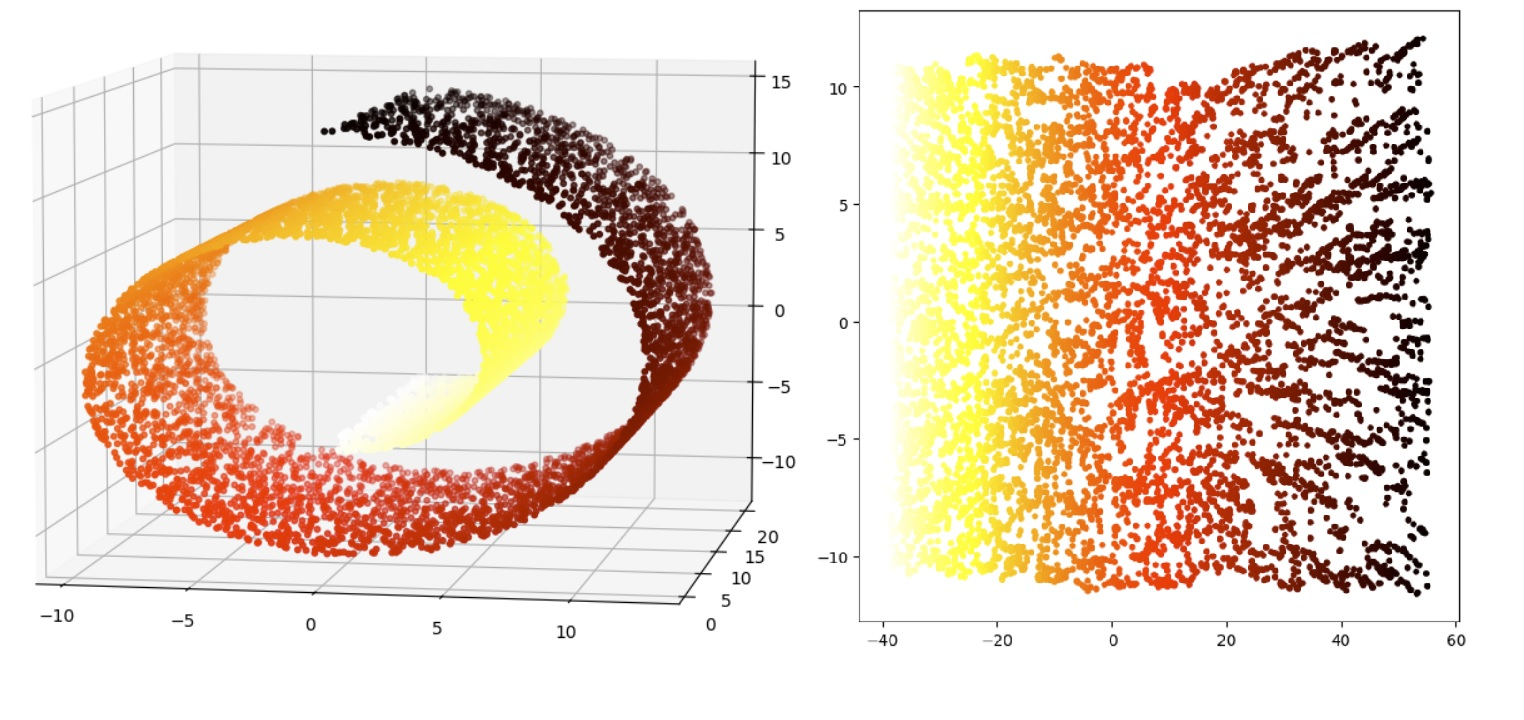
\includegraphics[width=14cm]{isomap.jpg}
    \caption{The input Swiss roll (left) and the output of Isomap (right). The Isomap successfully captures the nature of the manifold and "unrolls" the Swiss roll.}%
    \label{fig:isomap_swissroll}
\end{figure}

With the introduction of Isomap, it is easier to explain the drawbacks of LLE. As we can see in the steps of LLE, it emphasizes the local reconstruction of each data point using its neighbors. Because of this, LLE can potentially fail to preserve the global structure of the data, namely the distances on a larger scale. Points that are very far away in the original data set can be mapped close to one another in the output of LLE, especially when the space itself is very "curved". This shortcoming is addressed by Isomap, as the intermediate step of finding the graph $G$ is specifically designed to preserve global structure. Using MDS subsequently ensures that such preservation is translated into the low-dimensional output. The graph $G$ represents the grand picture Isomap tries to summarize.
\begin{figure}[ht]
    \centering
    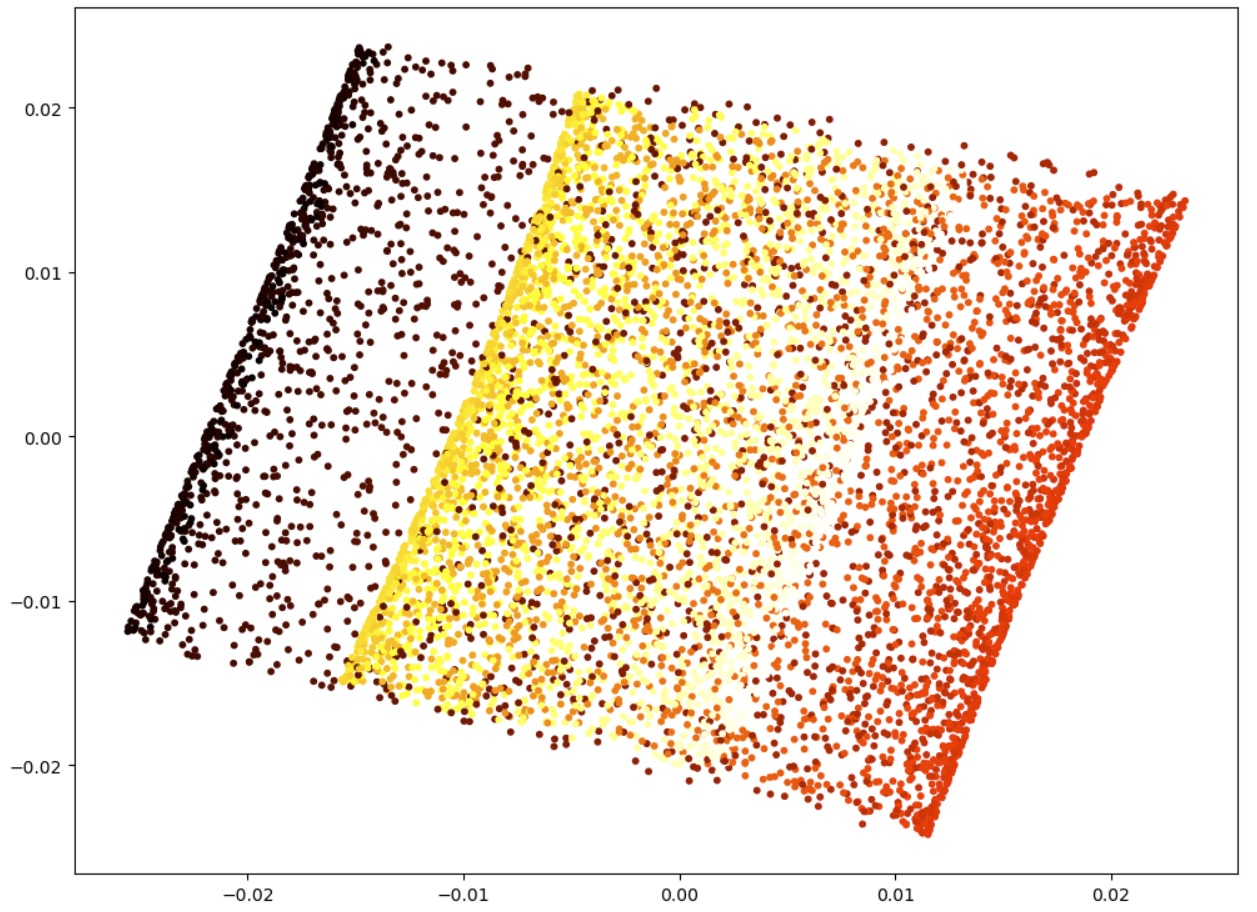
\includegraphics[width=10cm]{LLE_failed.jpg}
    \caption{A failed LLE output based on the same Swiss roll input in figure \ref{fig:isomap_swissroll}. The algorithm tries to search for neighbors in a overly broad area, causing the result to be distorted.}%
    \label{fig:lle_swissroll_failed}
\end{figure}
Nevertheless, Isomap is not perfect, either. As we already mentioned earlier in this section, MDS is a computationally expensive algorithm. On the top of that, given a graph $G = (V,E)$, the Dijkstra algorithm has a time complexity of $O(|E| + |V| \log |V|)$, where $|E|$ and $|V|$ are the number of edges and vertices in the graph respectively (\cite{Fredman1984fibonacci}). For dense graphs, $|E|$ will scale quadratically with $|V|$. By combining two computationally intense algorithms, Isomap is inevitably slow and becomes a bad choice for large and dense data sets.

Moreover, Isomap is very sensitive to the choice of hyperparameters and outliers. If the number of neighbors or the ball radius is too small, Isomap will sometimes produce a disconnected graph, prevents the algorithm from generating a global structure. But if the hyperparameters are too large, the algorithm might include "short-circuit" edges that connect points across gaps or folds in the manifold that are close in the ambient Euclidean space, such as distant points on a tightly packed Swiss roll. Then in this case Isomap will contain the worst of both worlds, by being an extraordinarily slow algorithm that also carries the disadvantages of LLE. Besides that, since Isomap is designed to preserve the global structure, it will cover everything, including outliers. Having an outlier in the data set, such as a point far away from everything else, can significantly disrupt the output.

Finally, Isomap carries some implicit assumptions. It assumes that the data on the manifold is well sampled, meaning that the graph constructed in Isomap is a truthful representation of the true geodesic distances on the manifold, from a differential geometry perspective. It also assumes that the intrinsic geometry of the manifold can be isometrically embedded into a lower-dimensional Euclidean space, hence the name. Such assumptions are not always true, and we should treat the output with caution if the stress values (similar to the definition in \eqref{strain_def}) are high.

Both LLE and Isomap are important milestones in the advancement of dimension reduction algorithms. With different focusing aspects, both provided us with a useful set of tools to analyze high-dimensional data, suited for different scenarios. However, mathematicians and computer scientists did not stop there. All the algorithms up to this point still work primarily with Euclidean distance. What if we want to extract the abstract structure of similarity out of the data sets, rather than the distance itself? What if we encode the information of neighborhood using probability distribution, rather than plain physical proximity? Such ideas inspired the creation of stochastic neighbor embedding (SNE) and the subsequent t-stochastic neighbor embedding (t-SNE). And that is where our story begins.
\subsection{The Road to t-SNE} \label{intro_chap:sec:tsne:preintro}
SNE was first introduced in 2002 by Hinton and Roweis (\cite{NIPS2002_6150ccc6}, with Roweis also being the creator of LLE). Like we just mentioned at the end of the previous section, SNE uses probability distributions to record the information of neighborhood. With this new framework, we need a new concept to measure the distance between two probability distributions, and that is the famous Kullback-Leibler (KL) divergence.
\begin{definition}
    Let $P$ and $Q$ be two probability measures with $p(x)$ and $q(x)$ as their respective probability density functions. The KL divergence between $P$ and $Q$ is defined as:
    \begin{align}
        D_{KL}(P||Q) = \int p(x) \log\left(\frac{p(x)}{q(x)}\right) dx.
    \end{align}
    In particular, if $P$ and $Q$ are discrete probability measures(distributions) defined on the same sample space $\mathcal{X}$, then the KL divergence is defined as:
    \begin{align}
        D_{KL}(P||Q) = \sum_{x \in \mathcal{X}} p(x) \log\left(\frac{p(x)}{q(x)}\right).
    \end{align}
\end{definition}
Note that the KL divergence is zero if and only if $P$ and $Q$ are the same distribution. At the same time, it is not symmetric and is not a true distance metric. It is also called the relative entropy. Since both SNE and t-SNE will construct probability distributions from the original data set, rather than plain Euclidean distance, KL divergence is used to formulate the loss function we aim to minimize.

SNE starts with defining the following probability mass function for each data point $X_i$: for each $j \neq i$, let
\begin{align}\label{SNE_input_kernel}
        p_{j|i} = \frac{\exp(-\norm{X_i - X_j}^2/2\sigma_i^2)}{\sum_{k \neq i}\exp(-\norm{X_i - X_k}^2/2\sigma_i^2)}.
\end{align}
$\sigma_i$ is a hyperparameter that is set by the user or by computation. We restrict that for each $i$, the induced probability distribution has the same entropy for all $i$. This means for some constant $\rho$, we have
\begin{align} \label{SNE_input_entropy}
    \sum_{j \neq i} p_{j|i} \log\left(p_{j|i}\right) = \log(N\rho),
\end{align}
where $N$ is the number of data points. The quantity $N\rho := \text{Perp}$ is called perplexity. This is a very clever design and it serves as a "slide bar" for each $X_i$. For example, the majority of the data points are located inside a ball with radius 1 and there is one data point that is more than 1000 units away. Then from that point's perspective, the rest of the data points are roughly "equally" distant from itself. The induced probability distribution will be very close to a discrete uniform distribution. A lot of information is lost during this process. By introducing perplexity, we allow each induced probability distribution to zoom in and out so that they are "observing" the rest from the data set on the same scale. Later we will see that this setting is not only backed up by clear intuition, but also plays an important role in proving the convergence to equilibrium measure in chapter 2, as well as in the prior work by Auffinger and Fletcher (\cite{auffinger-tsne}).

Let $Y_i$ be the low-dimensional output of SNE. We can define a similar probability mass function:
\begin{align} \label{SNE_output_kernel}
    q_{i|j} = \frac{\exp(-\norm{Y_i - Y_j}^2)}{\sum_{k \neq i}\exp(-\norm{Y_i - Y_k}^2)}.
\end{align}
Next, SNE will then try to minimize the KL divergence between the two (collections of) distributions, i.e.:
\begin{align} \label{SNE_loss_function}
    L = \sum_{i=1}^N D_{KL}(P_i||Q_i) = \sum_{i=1}^N \sum_{j \neq i} p_{j|i} \log\left(\frac{p_{j|i}}{q_{j|i}}\right). 
\end{align}
Since the input $X_i$'s are given and fixed, the loss function $L$ is a function of the output points $Y_i$'s. The minimum can be found using gradient descent. Different from LLE, SNE is not guaranteed to find a global minimum.

Though the formulation of SNE resembles LLE, the invention of SNE was still a refreshing evolution. From plain distance, to geodesic distance from constructed graphs, and now to probability distribution, it is good to see that mathematicians are using more flexible concepts to encode the general landscape of data. But people soon discovered that SNE has its own problems. Since the output distribution decays exponentially and it does not have a slide bar like perplexity, SNE is not able to distinguish clusters that are not in close proximity. This is the well-known "crowding problem" of SNE, and it directly inspired the birth the subsequent t-SNE algorithm (\cite{key}).

The t-SNE algorithm shares the same procedure as SNE. However, instead of using the Gaussian function in the output schema, t-SNE uses the much slower decaying student's t-distribution with 1 degree of freedom, i.e.,
\begin{align} \label{tSNE_output_kernel}
    q_{ij} = \frac{(1 + \norm{Y_i - Y_j}^2)^{-1}}{\sum_{k \neq i}(1 + \norm{Y_i - Y_k}^2)^{-1}}.
\end{align}
That is also where the letter "t" in the name comes from. The t-distribution greatly mitigates the crowding problem, and it is able to perform very well across different data sets. Also, t-SNE defines the input probability mass $p_{ij}$ as
\begin{align}
    p_{ij} = \frac{p_{j|i}+p_{i|j}}{2n},
\end{align}
which makes the input probability masses symmetric. One of the greatest and most well-known showcase of t-SNE is its implementation on the MNIST data set. The Modified National Institute of Standards and Technology (MNIST) is a large database consisting of handwritten digits. It is one of the mostly commonly used public data set for machine learning and computer vision. Started with USPS database that records handwritten zip codes, today's MNIST contains 60000 training images and 10000 testing images and serves as a benchmark for many machine learning algorithms. t-SNE is able to effectively capture the structure of data and clearly cluster different digits into separate groups. This algorithm is one of the greatest achievements in the field of dimension reduction and unsupervised learning in the 21st century.
\begin{figure}[h]
    \centering
    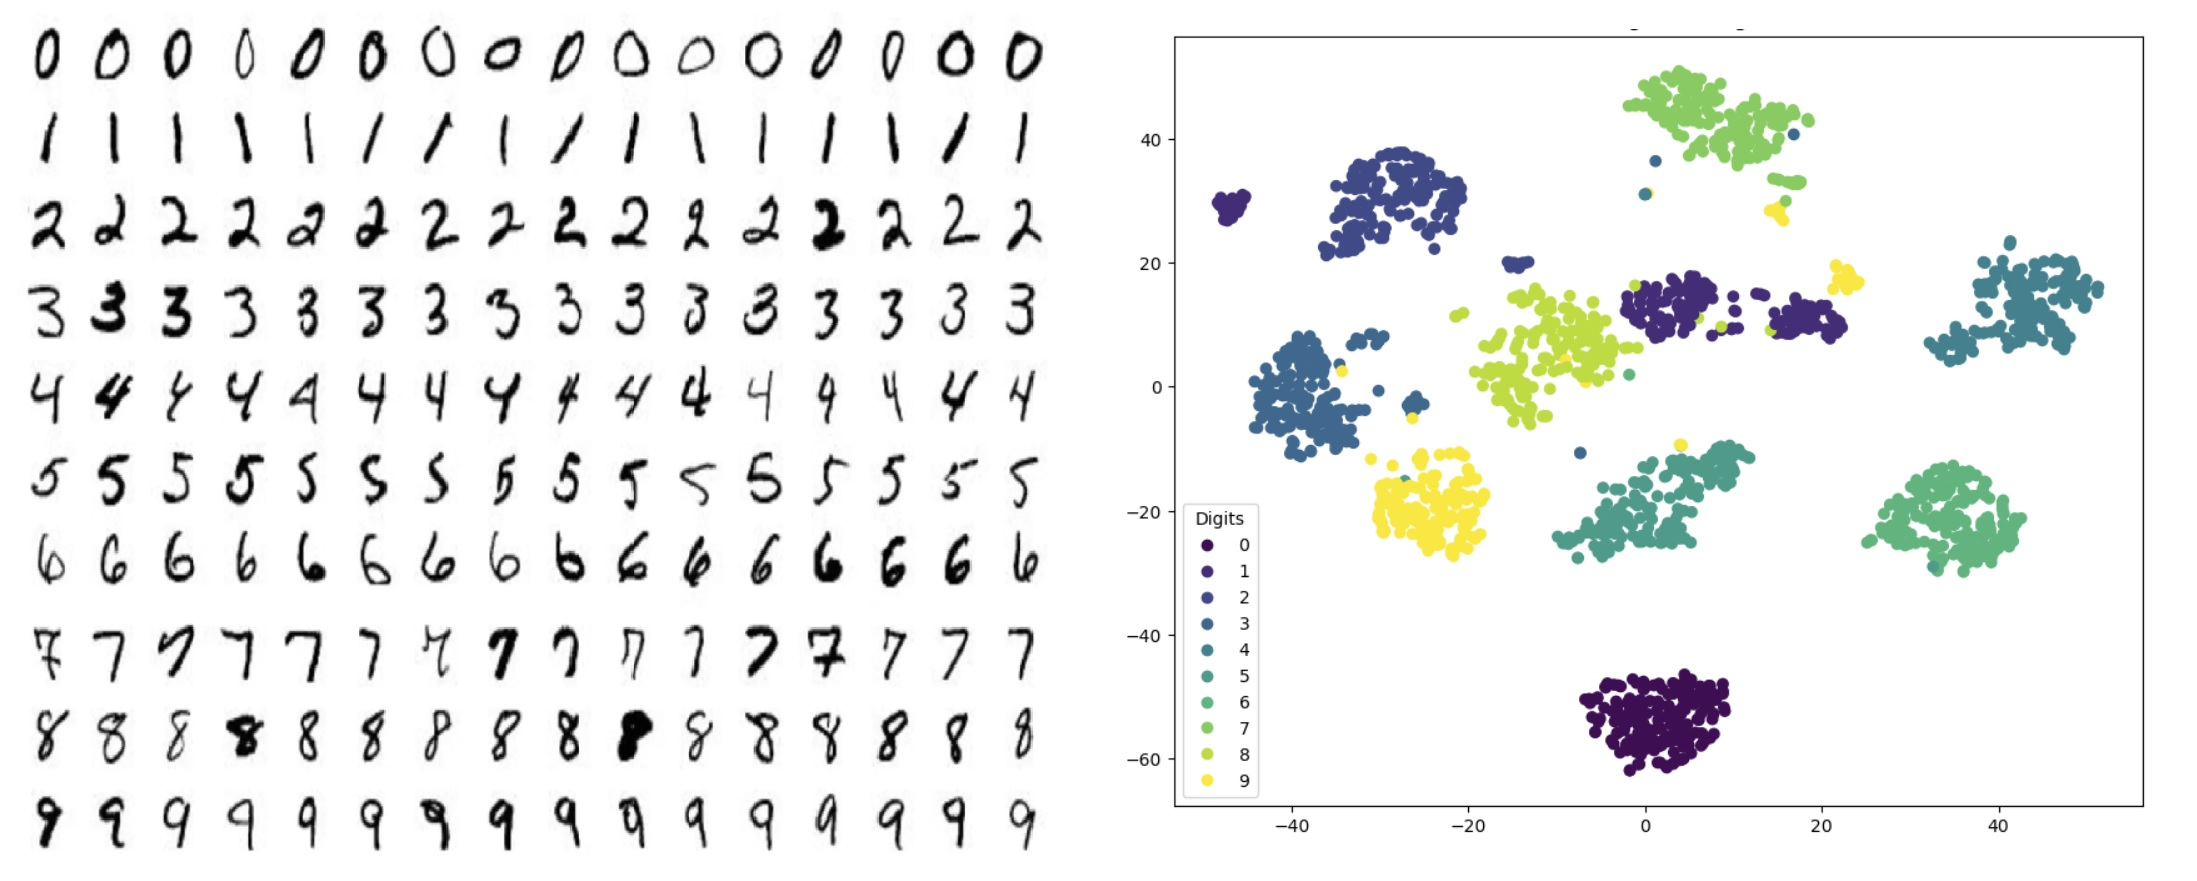
\includegraphics[width=14cm]{mnist_tsne.jpg}
    \caption{A sample of the MNIST dataset (left) and the output of t-SNE (right). t-SNE successfully grouped the handwriting with different digits together, with some minor imperfections (there are two clusters for the digit 0).}%
    \label{fig:mnist_tsne}
\end{figure}
Unfortunately, we need to repeat the same statement again: nothing is perfect. t-SNE is also a computationally expensive algorithm. If the data set is large and complex, it is advised to pre-process the data set using lightweight dimension reductions such as PCA. Meanwhile, though with better flexibility and overall performance, t-SNE inherits the same drawback from LLE: poor performance at preserving global structures. The distance between two clusters are often meaningless. We only know that the corresponding original data points do not belong to the same group, but little information can be extracted by the distance between the resulting low-dimensional clusters. t-SNE is also non-deterministic by nature: ending results might vary slightly for the same data set and hyperparameters. While the general cluster structures might be similar, the exact positions and orientations can vary, which can be sometimes confusing.

Such traits of t-SNE inspired some discussion regarding the mathematical nature of the algorithm. First, if t-SNE is non-deterministic, can we say something about its convergence and asymptotic behavior? Will the output of t-SNE converge to a certain equilibrium measure as we increase the number of samples to infinity? The answer is yes. We have the following results from \cite{auffinger-tsne}:

\begin{theorem} [Theorem 1.1, \cite{auffinger-tsne}] \label{thm:auffinger-tsne_1.1}
    Assume all input data points of t-SNE are drawn independent from a probability measure $\mu_X$. $\mu_X$ has a $C^1$ density function $f(x)$ and compact support. Denote $X$, $Y$ the input and output data set, $n$ the number of data points, $\rho$ the perplexity, and $L_{n,\rho}(X,Y)$ the loss function (KL-divergence) of t-SNE.
    
    Then for any $\rho \in (0,1)$ given, there exists a function $I_{\rho}$ and a set of measures $\mathcal{P}_{\mu_X}$, such that
    \begin{align}
        \lim_{n \to \infty} \inf_{Y} L_{n,\rho}(X,Y) = \inf_{\mu \in \mathcal{P}_{\mu_X}} I_{\rho}(\mu).
    \end{align}
\end{theorem}
If we write
\begin{align}
    \mu_n = \frac{1}{n}\sum_{i=1}^n \delta_{X_i,Y_i}
\end{align}
as the empirical measure of the input and output data set, then the following theorem also holds:
\begin{theorem}[Theorem 1.2, \cite{auffinger-tsne}] \label{thm:auffinger-tsne_1.2}
    Assume the same conditions as in theorem \ref{thm:auffinger-tsne_1.1}. Then there exists a measure $\mu^*$ and a sub-sequence $\{n_k\}$ such that $\mu_{n_k}$ converges weakly to $\mu^*$, and $\mu^* = \inf_{\mu \in \mathcal{P}_{\mu_X}} I_{\rho}(\mu)$. Moreover, $\mu^*$ has compact support.
\end{theorem}
The formulation of the theorems are slightly different from the original paper and some technical details are omitted due to the introductory nature of this chapter. The above two theorems send a strong message about the theoretical guarantee of t-SNE. If the input data is drawn independently from the same distribution, t-SNE is able to output a global minimum equilibrium measure (here measure means the distribution of the output data set) as we increase the sample size to infinity, with compact support. These are the first rigorous mathematical results about this algorithm after it has been used for so many years. And it leads to the next question, the question we are able to address in chapter 2. 

For the output distributions, using the Gaussian is not necessary as the successful execution of the algorithm does not rely on the specific properties of Gaussian functions. The two theorems above further verify this observation. This gives rise to the concept of kernels. For a pair of points $(x,y)$, a kernel is a positive function of $\norm{x-y}$ that we can use to determine the normalizing weights that produce the input and output distributions. For input, the kernel is the Gaussian function and for the output, the kernel is the function $f(x) = (1 + x^2)^{-1}$. It is natural to ask:

\textbf{``Is the student t-distribution not the only kernel that might give us the same theoretical guarantees? If no, then what is the class of output kernels that will give us the same results in \cite{auffinger-tsne}? Even more generally speaking, if we swap out both input and output kernels, what conditions do we need for the same theorems to be true?"}

These are the exact questions we are able to answer with rigorous proofs in chapter 2. Besides that, people are already swapping out output kernels in practice. Note that in the formula of KL-divergence, for the term $p_{ij}\log(p_{ij}/q_{ij})$ reaches its minimum zero when $p_{ij} = q_{ij}$. This means if we manually increase $p_{ij}$, the gradient descent process will tend to increase $q_{ij}$ as well. This is achieved by putting the output points $Y_i$ and $Y_j$ closer together, as the output kernel $f(x) = (1 + x^2)^{-1}$ is monotone decreasing. Therefore, in application people often replace $p_{ij}$ with its multiple $kp_{ij}$ for some constant $k > 1$. This is called the early exaggeration, one of the frequently used techniques. Using early exaggeration will result in closer clusters, improving visualization results.

Another known modification of the t-SNE algorithm is the heavy-tailed t-SNE. Recall that the density function of the t-distribution is given by
\begin{align} \label{t_dist_density}
    f(x) = \left(1+\frac{x^2}{\alpha}\right)^{-\frac{\alpha+1}{2}},
\end{align}
where $\alpha$ is the degree of freedom. Decreasing $\alpha$ will reduce its decaying speed and make it more "heavy-tailed". This will make $q_{ij}$ relatively larger and the output clusters will be compact. It is also shown in \cite{Kobak_2020} that heavy-tailed t-SNE tends to produce finer clusters, such as sub-clusters of the same digit in the MNIST data set.
\begin{figure}[ht]
    \centering
    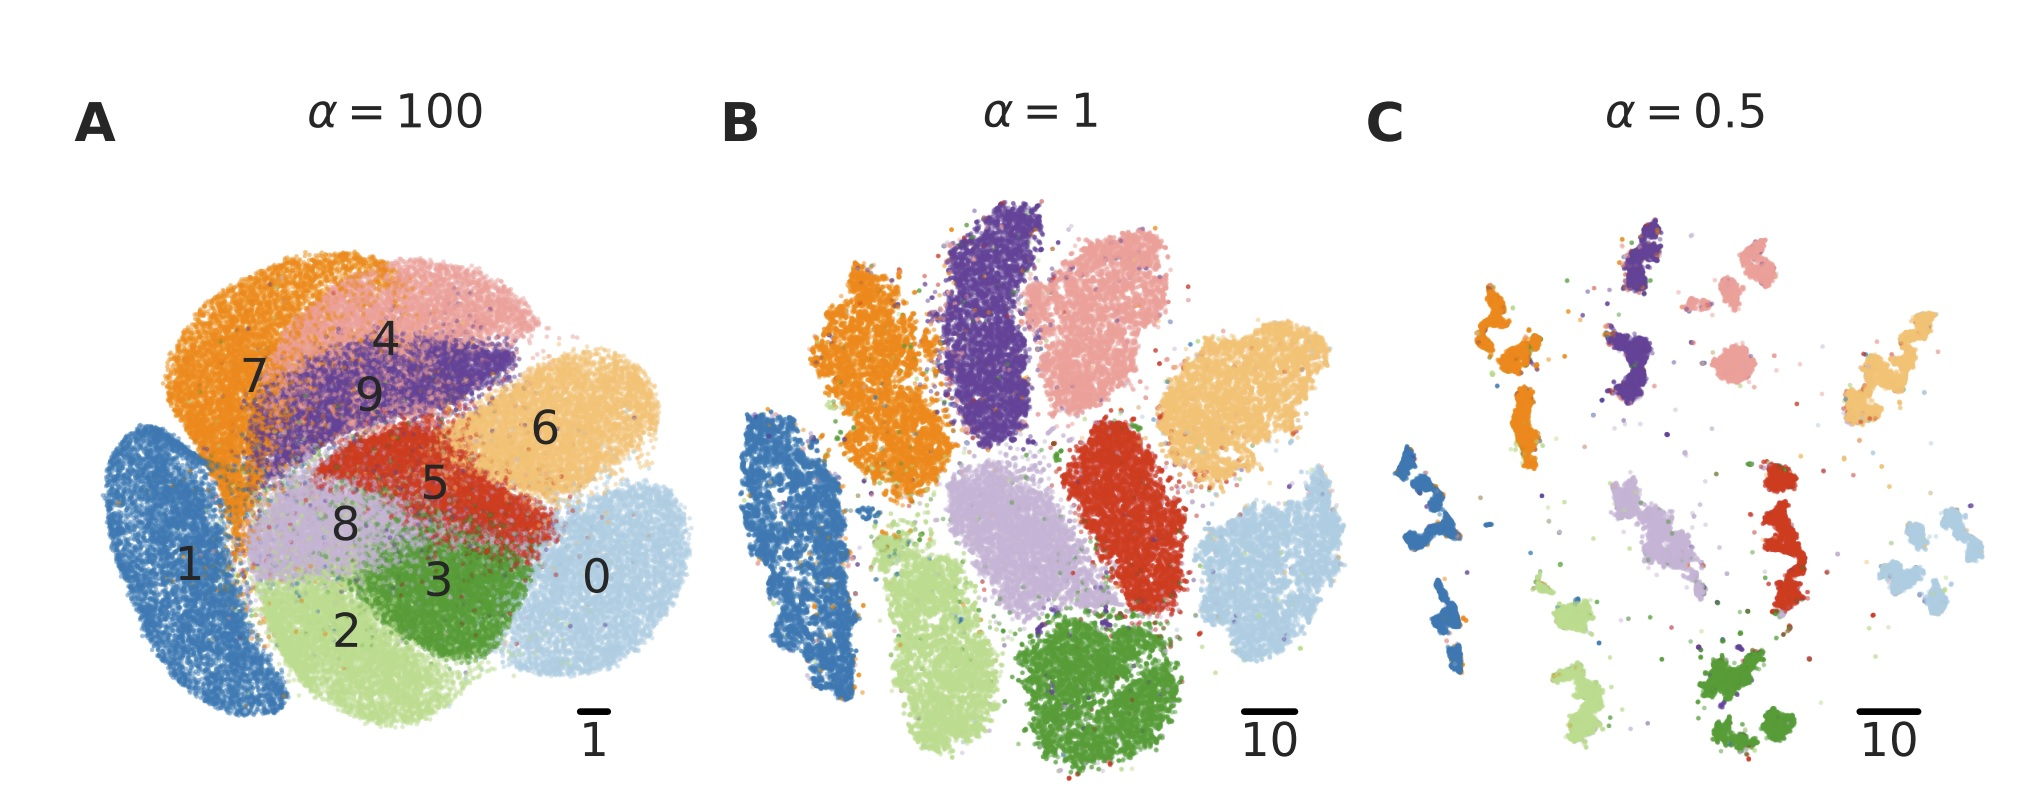
\includegraphics[width=14cm]{heavytail_tsne.jpg}
    \caption{The running result of different SNE algorithms in \cite{Kobak_2020}, with (A) being the light-tail t-SNE, (B) the normal t-SNE and (C) the heavy-tailed t-SNE. Heavy tailed variants are producing tighter and finer clusters, while the light-tail version produces results similar to the original SNE. ($t$-distribution will converge to Gaussian if $\alpha \to \infty$.)}%
    \label{fig:heavytail_tsne}
\end{figure}
Both early exaggeration and heavy-tailed t-SNE can be seen as manipulations of the output kernel. t-SNE works effectively under the modification and produces promising results, besides different characteristics researchers hope to see. Besides exploring different conditions for the convergence to hold and the equilibrium measure to exist, it is also an interesting problem to see how exactly the output changes with the modification of the output kernel. Some insightful results can be found in \cite{weinkove2024flow}.

It is fascinating to see the rigorous mathematical theory behind widely used algorithms like t-SNE, which are often used to produce qualitative rather than quantitative results. Getting to the bottom of the convergence behavior will provide valuable insights on the algorithm itself, refining the theoretical landscape of the dimension reduction theory. We will resume our journey in chapter 2.